%! Author = naza
%! Date = 3/10/25

% Preamble
\documentclass[a4paper,oneside,12pt]{amsart}

% Packages
\usepackage{amsmath}
\usepackage{latexsym}
\usepackage{multicol}
\usepackage{enumerate}
\usepackage{enumitem}
\usepackage[heightrounded]{geometry}
\geometry{top=2cm,bottom=2cm,left=2cm,right=2cm}
\usepackage{graphicx}
\newcommand{\xopt}{x^{*}}
\newcommand{\yopt}{y^{*}}
\newcommand{\zopt}{z^{*}}
\theoremstyle{definition}
\newtheorem{quest}{Ejercicio}
\thispagestyle{empty}
\usepackage{tikz}
\usetikzlibrary{automata,positioning}

% Document
\begin{document}

    \begin{quest}
        \item \begin{enumerate}[label=\alph*)]
                  \item
                  \[
                      \begin{array}{rclllll}
                          w_2 & =  &6 &-x_1 &  &-2x_3 & \\
                          a_1 & =  &4 &-x_1 &-x_2 &-x_3 &+w_1\\
                          a_2 & =  &2 &+x_1 &-x_2 &-x_3 & \\\hline
                          z &= &-6M &+2x_1 &+(M+1)x_2 &+(M+1)x_3 &-Mw_1\\
                      \end{array}
                  \]
                  \vspace{1cm}

                  \[
                      \begin{array}{rclllll}
                          w_2 & =  &6 &-x_1 &-2x_3 &  & \\
                          a_1 & =  &2 &-2x_1 &  &+w_1 &+a_2\\
                          x_2 & =  &2 &+x_1 &-x_3 &  &-a_2\\\hline
                          z &= &-(M-2) &+(2M+3)x_1 &  &-Mw_1 &-(2M+1)a_2\\
                      \end{array}
                  \]
                  \vspace{1cm}

                  \[
                      \begin{array}{rclllll}
                          x_2 & =  &3 &-x_3 &+1/2w_1 &-1/2a_1 &-1/2a_2\\
                          w_2 & =  &5 &-2x_3 &-1/2w_1 &+1/2a_1 &-1/2a_2\\
                          x_1 & =  &1 &  &+1/2w_1 &-1/2a_1 &+1/2a_2\\\hline
                          z &= &5 &  &+3/2w_1 &-(2M+3)/2a_1 &-(M-1)/2a_2\\
                      \end{array}
                  \]
                  \vspace{1cm}

                  \[
                      \begin{array}{rclllll}
                          x_1 & =  &6 &-2x_3 &-w_2 &  & \\
                          x_2 & =  &8 &-3x_3 &-w_2 &  &-a_2\\
                          w_1 & =  &10 &-4x_3 &-2w_2 &+a_1 &-a_2\\\hline
                          z &= &20 &-6x_3 &-3w_2 &-Ma_1 &-(M+1)a_2\\
                      \end{array}
                  \]

                  \vspace{1cm}
                  Valor óptimo de las variables básicas:
                  \[
                      \begin{array}{l}
                          x_1  = 6 \\
                          x_2  = 8 \\
                          w_1  = 10 \\
                      \end{array}
                  \]
                  Valor óptimo de la función objetivo: $20$
                  \item  Problema dual:
                  \[
                        \begin{array}{rrcrcrcr}
                            \min & 4y_1 & + & 6y_2 & - & 2y_3 & & \\
                            \text{s.a:} & y_1 & + & y_2 & + & y_3 & \geq & 2\\
                            & y_1 &  &  & - & y_3 & \geq & 1\\
                            & y_1 & + & 2y_2 & - & y_3 & \geq & 1\\
                            & \multicolumn{5}{r}{y_1} & \leq & 0 \\
                            & \multicolumn{5}{r}{y_2} & \geq & 0 \\
                            & \multicolumn{5}{r}{y_3} &  & \text{libre} \\
                        \end{array}
                        \]
                  \item Aplicamos Teorema de Holgura Complementaria:
                    \[
                  \begin{array}{rl}
                      x_1^\ast + x_2^\ast + \xopt_3 > 4 & \Rightarrow y_1^\ast = 0 \\
                      x_1^\ast \neq 0 & \Rightarrow \yopt_1+\yopt_2+\yopt_3 = 2 \\
                      \xopt_2 \neq 0 & \Rightarrow \yopt_1 - \yopt_3 = 1 \\
                  \end{array}
                  \]
                  Tenemos entonces que:
                  \[
                      \begin{cases}
                          -\yopt_3 = 1 \\
                          \yopt_2 + \yopt_3 = 2
                      \end{cases}
                      \Rightarrow \yopt = (0,-1, 3)
                  \]
        \end{enumerate}
    \end{quest}

    \begin{quest}\hphantom{1em}

        \begin{enumerate}
            \item Solución degenerada: la variable básica $x_3$ vale $0$.
            \item No acotado: si $x_5$ entra a la base, puede aumentar indefinidamente.
            \item Infinitas soluciones óptimas: $x_2$ puede tomar cualquier valor en $[0,8]$ y la solución sigue
            siendo óptima.
            \item Solución óptima única no degenerada: los costos reducidos son todos negativos.
        \end{enumerate}
    \end{quest}

    \begin{quest}\hphantom{1em}

        \textbf{Poliedro de la relajación lineal:}
        \begin{figure}[htbp!]
            \centering
            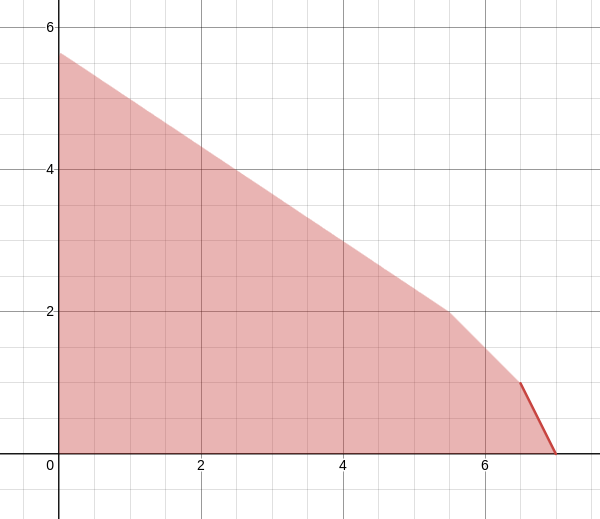
\includegraphics[width=0.5\textwidth]{grafico_BB_recu}
        \end{figure}

       \textbf{Árbol de B\&B:}

        \begin{figure}[htbp!]
            \centering
            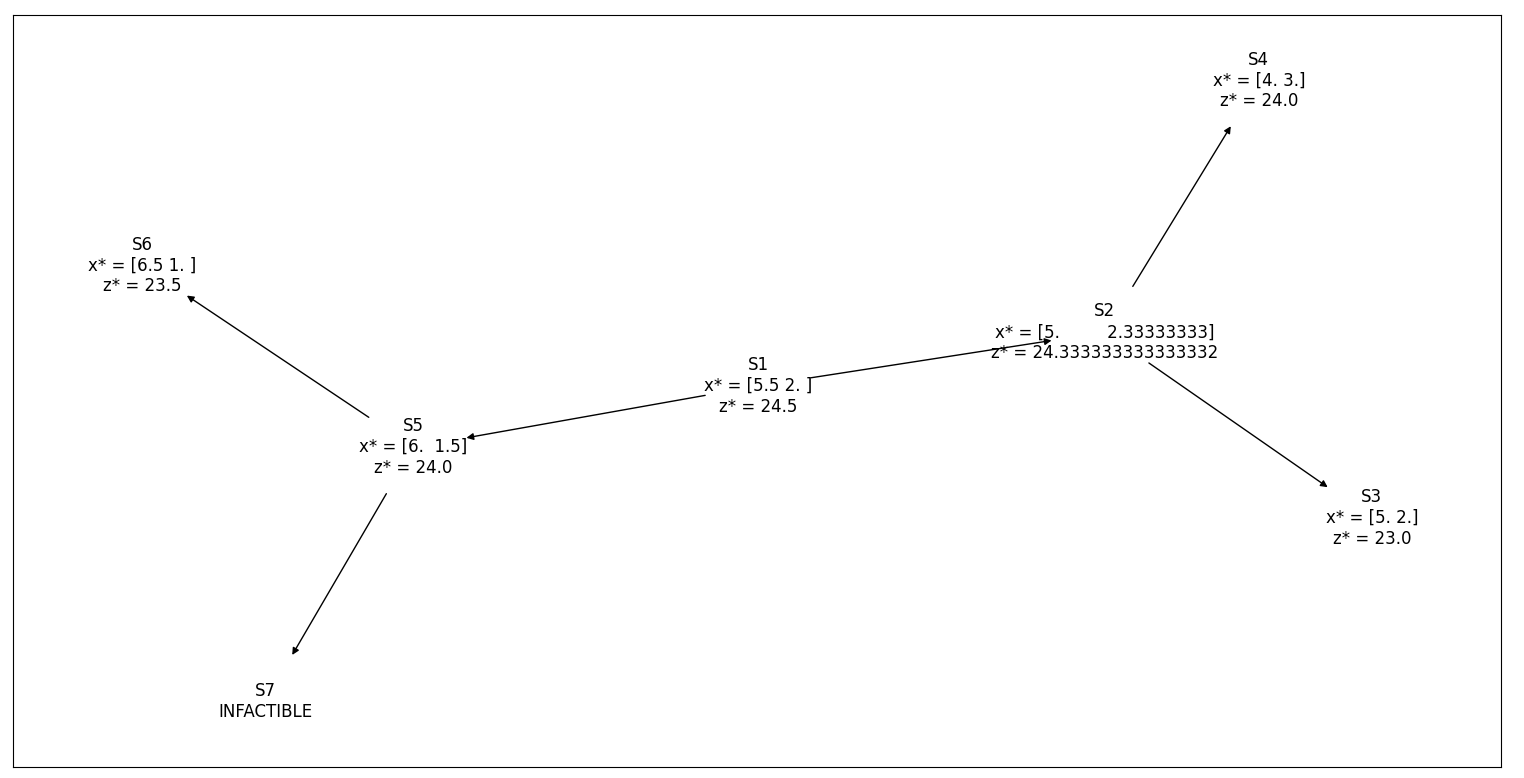
\includegraphics[width=\textwidth]{Arbol_BB_2do_recu}
        \end{figure}
    \end{quest}
\end{document}